\section{System Implementation and Specifications}

\subsection{Hardware Specifications}\label{hardware}
\subsubsection{Processing Hardware}
The current software implementation requires a simple processor but is constrained by its speed. The primary hardware limitation is the available RAM, with a recommended range of 2 to 4 GB for the planner, depending on the size of the input state configuration.
\\\\
During the project, system timing results were obtained using a general-purpose desktop computer with the following specifications:
\\
\begin{tabularx}{1\textwidth}{ p{0.22\textwidth} p{0.78\textwidth} }
	\textbf{Operating System:} 	& Windows 10 Pro 64-bit (10.0, Build 19045)\\
	\textbf{Processor:} 		& AMD Ryzen 7 3700X 8-Core (16 CPUs) clocked at approximately 3.6 GHz\\
	\textbf{GPU:} 				& NVIDIA GeForce RTX 2070 Super with 8GB VRAM\\
	\textbf{RAM:} 				& 3 x 8 GB DDR4 Memory clocked at 3200 MHz\\
	\textbf{Memory:} 			& 1 TB M.2 SSD with read speeds of 7,300 MB/s and write speeds of 540 MB/s\\
\end{tabularx}

\subsubsection{Mobile Manipulator}
The mobile manipulator available in the lab is the Automata EVA, further details can be seen in \nameref{evaSpecSheet}. The manipulator was not physically used during the project due to time constraints. Though, the arm specifications were used for simulation so the current state of the reconfiguration planner can be integrated with the arm in a future project.

\subsection{Software Specifications}
\subsubsection{Software Architecture Overview}
\begin{figure}[H]
	\centering
	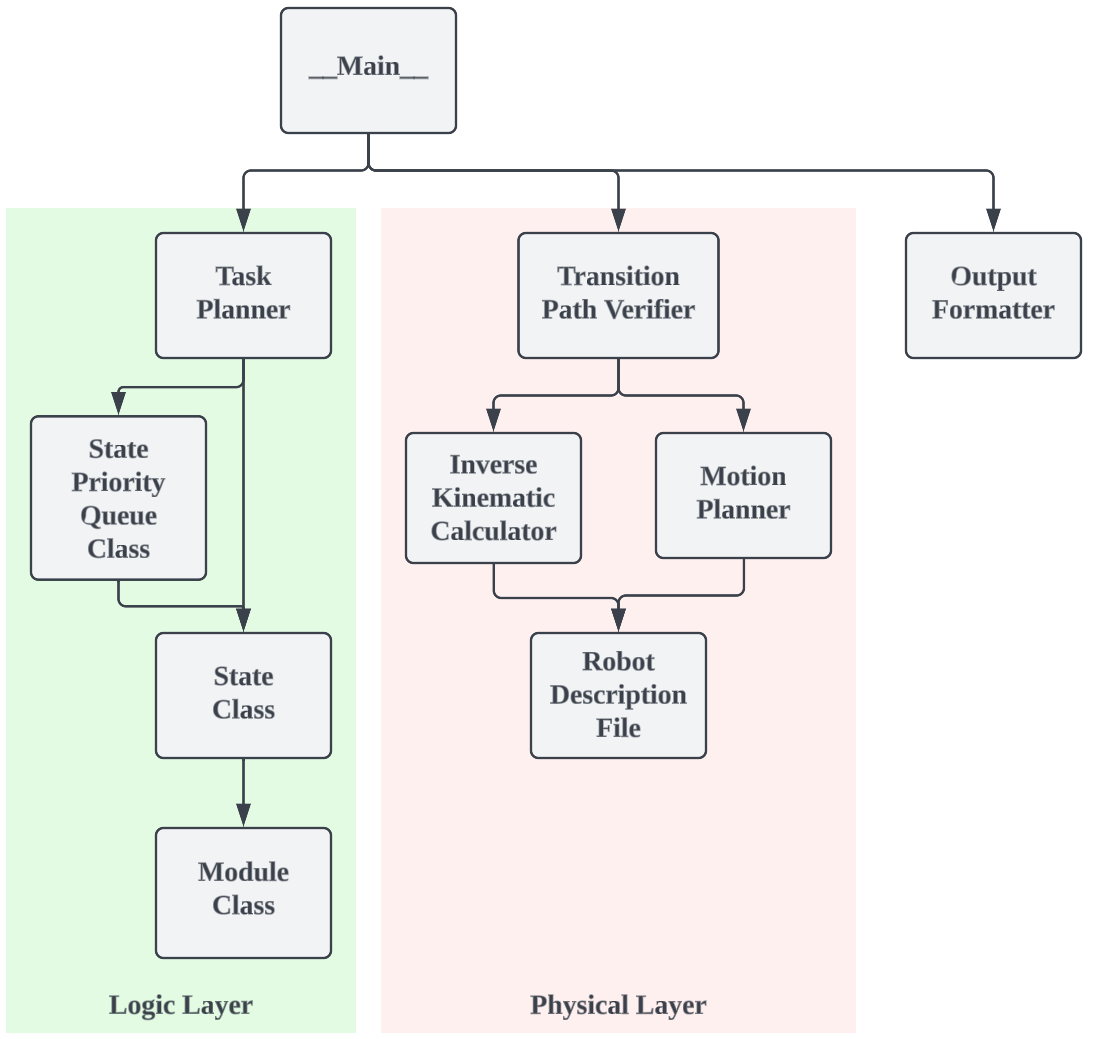
\includegraphics[width=\textwidth]{softwareImplementation.png}
	\caption{High-level System Implemented Design}
	\label{systemImplementation}
\end{figure}
The modular structure of the final software implementation is illustrated in Figure \ref{systemImplementation}. The main file integrates the Logic Layer and Physical Layer, facilitating communication and applying feedback strategies between them. Once a solution is found, the Output Formatter is used to display the instructions to users (seen in \nameref{5modTest}) and to create animations of state reconfiguration transitions for visual analysis of the process.

\subsubsection{Logic Layer - Overview}
The Logic Layer consists of a Task Planner and its related methods, and classes to implement States, Modules and State Priority Queues

\subsubsection{Logic Layer - Task Planner}
The Task Planner begins by verifying the start and goal states have the same number and composition of modules; And generates states utilising the State Priority Queue and State Classes. It returns an array of states representing the transitions required to reconfigure the start state into the goal state.
\\\\
The Planner consists of two main methods, \textbf{“FindPath()“} and \textbf{“GenNewStates()”}. The \textbf{“FindPath()“} method implements the search algorithm shown in listing \ref{SearchPseudo}), while \textbf{“GenNewStates()”} expands the tree based on the heuristics specified in the design section \ref{genStates},a as can be seen in listing \ref{generateStatesPseudo}. After generating states, “FindPath()” records their parent states, enabling the program to trace the transition path from the starting state to the goal state.

\begin{lstlisting}[caption={State Generation Pseudo-code},captionpos=b,label={generateStatesPseudo}]
GenNewStates(state, goalState)
	stateQueue <- new StateQueue(goalState) 
	from <- state.getNonFinalModules()
	to <- state.getAvailablePositions()
	
	stateQueue.push(state.GenerateMoves(from, to))
	
	IF stateQueue.empty() DO:
		from <- state.getAdjacentModules(b)
		stateQueue.push(state.GenerateMoves(from, to))
	END
	
	IF stateQueue.empty() DO:
		from <- state.getModules()
		stateQueue.push(state.GenerateMoves(from, to))
	END
	RETURN stateQueue
\end{lstlisting}

\subsubsection{Logic Layer - State Priority Queue Class}
The State Priority Queue class maintains a sorted list of states using a simple array data structure. States are ordered based on their proximity to the goal state, as determined by the heuristics detailed in design section \ref{statePriority}. When a state is inserted, a binary search algorithm \cite{lin2019binary} is used to find the appropriate position in the queue to maintain the queue's priority order. Initially, a linear search algorithm was used for simplicity, but during optimization, the binary search was implemented, significantly reducing the overall insertion time.

\subsubsection{Logic Layer - State Class}
The State Class represents a state configuration and stores module positions. It includes methods for state comparisons, measurements, validation, and visualization. Modules are stored in a dictionary, where keys represent module positions and values are module objects.
\\\\
Initially, a position matrix was used for its simplicity in testing and modifying logic, which sped up development. However, it was later replaced by a dictionary for optimisation as unlike a position matrix, dictionaries do not store unnecessary zero values so increase memory efficiency of the system.
The class includes a verification function to ensure all modules in the state are connected.
\\\\
Originally, an out-of-the-box labelling algorithm from the scikit-image python package \cite{scikit-image} was used with the position matrix to verify connectivity. After switching to a dictionary, a new search algorithm was implemented for state verification (shown in listing \ref{verifyPseudo}).
\\\\
\begin{lstlisting}[caption={State Verification Pseudo-code},captionpos=b,label={verifyPseudo}]
VerifyState(state)
	foundList <- []
	searchList <- [state.getFirstModule()]
	WHILE searchList NOT empty DO:
		module <- searchList.pop()
		For neighbour in module.getNeighbours() DO:
		IF neighbour NOT in foundList DO:
			IF neighbour NOT in searchList DO:
				searchList.push(neighbour)
			END
		END
	END
	RETURN foundList.length() EQUALS state.numModules()
\end{lstlisting}
Several functions are implemented to measure the number of modules in final positions, the number of modules in free positions and the Euclidean distance between all modules in non-final positions and their final positions. Since these measurements are often requested multiple times for the same state, the calculated values are saved within the state after the initial computation and updated only if the goal state changes.
\\\\
For visualising reconfigurations and aiding in-depth testing and analysis, the State Class includes a display function. This function translates the dictionary into a position matrix, which is then displayed as a 3D matrix using Matplotlib \cite{Hunter2007}. Configurations, such as the one shown in figure \ref{stateVisual}, can be visualised. Additionally, this function is used to create reconfiguration videos, enabling clear visualisation of the system's output.
\begin{figure}[H]
	\centering
	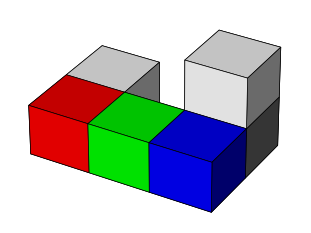
\includegraphics[width=0.5\textwidth]{state.png}
	\caption{State Visualisation}
	\label{stateVisual}
\end{figure}

As shown in listing \ref{generateStatesPseudo}, the State Class includes a function called \textbf{'GenerateMoves()'} for generating a list of states for mass movement of modules. This function takes two lists: one of module positions and another of positions the modules can move to. For each module, the function validates the state without the moving module to ensure the state remains intact during movement. It then moves the module to each of the possible positions, adding the new state to a return list if the state is valid after the movement. This custom mass movement function optimizes state generation during search tree expansion.

\subsubsection{Logic Layer - Module Class}
The Module Class is a straightforward class that holds information about a module, primarily used for comparing modules through an \textbf{"Equals()"} function. This function can be modified to adjust which module properties determine equality. In its current implementation, colour is used to decide if two modules are equal. There is functionality to compare by module type or module identification number. However, comparing by colour simplifies analysis during testing, as it allows for visual differentiation of modules when displayed.
\subsubsection{Physical Layer - Inverse Kinematics Verifier}
As detailed in design section \ref{IKDESIGN}, the implemented Inverse Kinematics Verifier uses an analytical solution to calculate the manipulator joint angles required to position the end-effector at a specified location. Initially, an analytical formula was developed specifically for the Automata EVA arm (details in \nameref{evaSpecSheet}) available in the lab. This limited the compatibility of the reconfiguration planner to only that specific manipulator.
\\\\
To increase compatibility, a Unified Robotics Description Format (URDF) file was created for the Automata EVA, as shown in \nameref{evaURDF}. The IKPy package \cite{ikpy} was then used to generate an analytical solution for use by the Inverse Kinematics Verifier and Motion Planner. Users can now update the reconfiguration planner to work with different mobile manipulators by simply replacing or modifying the URDF file.
\\\\
The inverse kinematics verifier is used to ensure that the start and final position of each module movement in the reconfiguration semantic solution is reachable by the mobile manipulator. In the case of a module being out of reach, the verifier returns the state transition that caused the failure. Otherwise, the semantic solution is sent to the motion planner for further processing.

\subsubsection{Physical Layer - Robot Description File}
\begin{figure}[H]
	\centering
	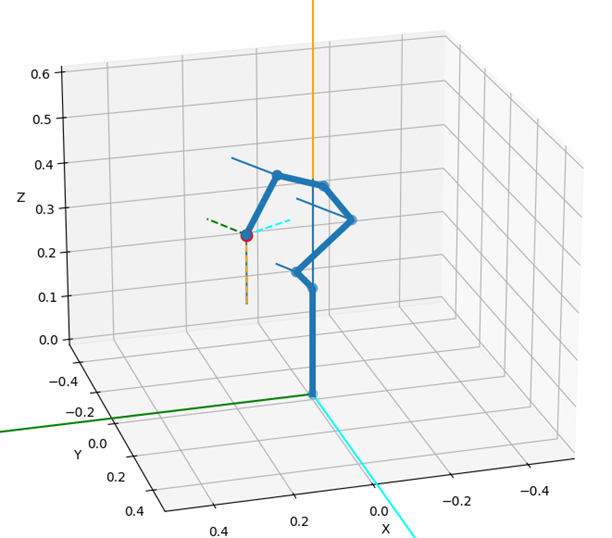
\includegraphics[width=\textwidth]{IK.png}
	\caption{Automata EVA Kinematics Visualisation}
	\label{EvaIKbasic}
\end{figure}
A URDF file is used to define the mechanical structure, dimensions, joint configurations, and physical constraints of the mobile manipulator the physical layer is simulating to verify the logic layers semantic solution. URDF files are an XML-based file format that is widely used in robotics \cite{urdfProof} to describe robots to software systems. The file describes a robot as a collection of links and joints that can articulate around each other according to specified constraints. URDF files are also modular meaning they can include other URDF files, aiding in the design of particularly complex robots. This for example means that a user can develop a URDF file for an arm end-effector and simply include it in the already existing arm file to attach it to the arm. 
URDF files also allow for the visualization of the defined arm joints, as seen in figure \ref{EvaIKbasic} which can be overlaid on top of our module state display to visualise mobile manipulator pose on the modular space system. Additionally available online packages such as urdf-loader \cite{urdfLoader} can display the visual meshes described in the URDF file to view the mobile manipulator in more detail such as seen in figure \ref{EvaIKadvanced}.
\begin{figure}[H]
	\centering
	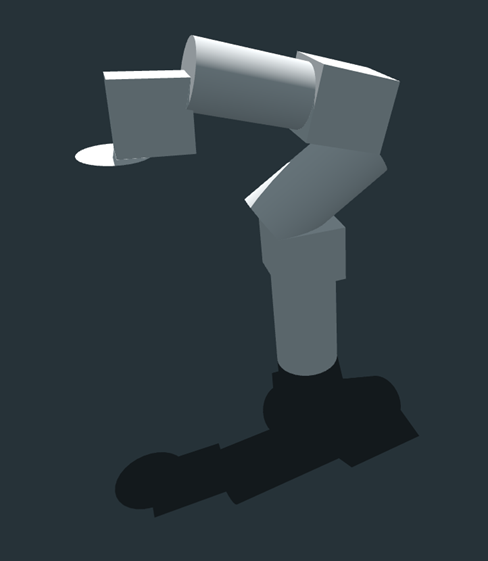
\includegraphics[width=0.8\textwidth]{IKmodel.png}
	\caption{Automata EVA URDF Model Visualisation created through urdf-loader \cite{urdfLoader}}
	\label{EvaIKadvanced}
\end{figure}

\subsubsection{Physical Layer - Motion Planner}
Due to time constraints during the project, instead of implementing an advanced motion planner, a simple motion planner was implemented that makes assumptions based on the lab environment surrounding the mobile manipulator available in the lab. Physical constraints of the robot arm and the environment are applied to the system during module movements using 2 basic rules:
\begin{enumerate}[]
	\item Modules can only be picked up by the mobile arm if no blocks are above them.
	\item Modules can only be placed at a supported position (above another module and on the ground) and cannot be placed at negative z values (below the ground)
\end{enumerate}
The combination of these two rules applies the physical constraints of gravity and the presence of the ground. If either rule is broken, the planner returns the state transition causing the failure. Otherwise, it generates and returns an instruction set in the form of an array containing each manipulator action sequentially required to perform the state reconfiguration. The available instructions the motion planner can generate can be seen in Figure \ref{instructions}

\begin{figure}[H]
	\begin{tabularx}{\textwidth} {| p{0.16\textwidth} | p{0.14\textwidth} | X |}
		\hline
		\textbf{Instruction} & \textbf{Information} & \textbf{Action}\\
		\hline
		CONNECT 	 & None	& Signal the arms end-effector to grab/connect\\
		\hline
		DISCONNECT   & None & Signal to the arms end-effector to drop/disconnect\\
		\hline
		MOVE TO 	 & Position, Joint angles & Move the arm to position the end-effector at the supplied position by transitioning the arms joint angles to the supplied joint angles\\
		\hline
	\end{tabularx}
	\caption{Instructions available to the Physical Layer Motion Planner}
	\label{instructions}
\end{figure}



\subsection{Feedback Strategies}
Currently, the system employs a basic feedback strategy. Upon detecting a failure in the physical layer, the system returns the state transition responsible for the failure. Subsequently, the branch of the tree originating from the failing state transition is removed, eliminating states where the failing state was as an ancestor. The pruned search tree is then passed back to the logic layer to pursue an alternative semantic solution.

\input{sections/Implementation/Challenges}

